\documentclass[10pt]{book}
%\documentclass[10pt]{book}
\def\baselinestretch{1.1}
\usepackage[bookmarks]{hyperref}
\usepackage{kotex} % korean tex
\usepackage[utf8]{inputenc} % set input encoding (not needed with XeLaTeX)
\usepackage{framed}
%-----Insert Fortran code 
\usepackage{listings}
\lstset{language=[90]Fortran,
  basicstyle=\ttfamily,
  keywordstyle=\color{red},
  commentstyle=\color{green},
  morecomment=[l]{!\ }% Comment only with space after !
}
% Fortran code example
%\begin{lstlisting}[frame=single]
%! Der folgende Fortran-Code ist bei Wikipedia geklaut.
%SUBROUTINE test( Argument1, Argument2, Argument3 )
%   REAL,              INTENT(IN) :: Argument1
%   CHARACTER(LEN= *), INTENT(IN) :: Argument2
%   INTEGER,           INTENT(IN), OPTIONAL :: Argument3
%   ! This makes sense
%END SUBROUTINE
%\end{lstlisting} 
%-----------------------------
\usepackage{geometry} % to change the page dimensions
\geometry{letterpaper} % or letterpaper (US) or a5paper or....
% \geometry{margins=2in} % for example, change the margins 
%to 2 inches all round
% \geometry{landscape} % set up the page for landscape
%   read geometry.pdf for detailed page layout information

\usepackage{graphicx} % support the \includegraphics command and options

% \usepackage[parfill]{parskip} % Activate to begin paragraphs 
%with an empty line rather than an indent

\usepackage{booktabs} % for much better looking tables
\usepackage{array} % for better arrays (eg matrices) in maths
\usepackage{paralist} % very flexible & customisable lists 
%(eg. enumerate/itemize, etc.)
\usepackage{verbatim} % adds environment for commenting 
% out blocks of text & for better verbatim
\usepackage{subfig} % make it possible to include 
%more than one captioned figure/table in a single float
% These packages are all incorporated in the memoir class 
%to one degree or another...

%%% HEADERS & FOOTERS
\usepackage{fancyhdr} % This should be set 
% AFTER setting up the page geometry
\pagestyle{fancy} % options: empty , plain , fancy
\renewcommand{\headrulewidth}{0pt} % customise the layout...
\lhead{}\chead{}\rhead{}
\lfoot{}\cfoot{\thepage}\rfoot{}

%%% SECTION TITLE APPEARANCE
\usepackage{sectsty}
\allsectionsfont{\sffamily\mdseries\upshape} 
% (See the fntguide.pdf for font help)
% (This matches ConTeXt defaults)

%%% ToC (table of contents) APPEARANCE
\usepackage[nottoc,notlof,notlot]{tocbibind} 
% Put the bibliography in the ToC
\usepackage[titles,subfigure]{tocloft} 
% Alter the style of the Table of Contents
\renewcommand{\cftsecfont}{\rmfamily\mdseries\upshape}
\renewcommand{\cftsecpagefont}{\rmfamily\mdseries\upshape} % No bold!

\usepackage{amsmath}
\usepackage{amssymb}
\usepackage{epsfig}
\usepackage{color}

\usepackage{empheq}
% make possible to box equations, For example
%\begin{empheq}[box=\fbox]{align*}
%a&=b \tag{test}\\
%E&=mc^2 + \int_a^a x\, dx
%\end{empheq}

\parindent 10pt\textheight 9in\topmargin -0.4in\textwidth 6in
\oddsidemargin .25in\evensidemargin 0in
\def\bm{\boldsymbol}
\newcommand{\bea}{\begin{eqnarray}}
\newcommand{\eea}{\end{eqnarray}}
\newcommand{\be}{\begin{eqnarray}}
\newcommand{\ee}{\end{eqnarray}}
\newcommand{\no}{\nonumber \\}
\newcommand{\nnb}{\nonumber}
\newcommand{\etal}{{\it et al.}~}
\newcommand{\eg}{{\it e.g.}}
\newcommand{\ie}{{\it i.e.}}
\newcommand{\sll}[1]{#1\hspace{-0.5em}/}
\newcommand{\del}{\partial}
\def\vs{{\bm \sigma}}

\def\vh{{\bm h}}
\def\vk{{\bm k}}
\def\vl{{\bm l}}
\def\vm{{\bm m}}
\def\vn{{\bm n}}
\def\vp{{\bm p}}
\def\vq{{\bm q}}
\def\vr{{\bm r}}
\def\vR{{\bm R}}
\def\vv{{\bm v}}
\def\vx{{\bm x}}
\def\vy{{\bm y}}

\def\la{\langle}
\def\ra{\rangle}
\newcommand{\threejsymbol}[6]
{\left(\begin{tabular}{ccc} {$#1$}&{$#2$}&{$#3$}\\
                             {$#4$}&{$#5$}&{$#6$}\end{tabular}\right)}
\newcommand{\sixjsymbol}[6]
{\left\{\begin{tabular}{ccc} {$#1$}&{$#2$}&{$#3$}\\
                             {$#4$}&{$#5$}&{$#6$} \end{tabular}\right\}}


%%% The "real" document content comes below...

\title{Lattice EFT note 2: projectMC code}
\author{Young-Ho Song}
\date{\today}
%\date{} % Activate to display a given date or no date (if empty),
         % otherwise the current date is printed 

\begin{document}
\maketitle
\tableofcontents

\newpage
\chapter{Introduction on numerical code}
Let us roughly summarize the numerical procedure to compute any observable in lattice EFT. 

The basic quantity in NLEFT is 
\bea 
Z(T)=\int {\cal D} c{\cal D} c^* \exp(-S[c,c^*]) 
\eea 
with appropriate boundary conditions on $c, c^*$. 
By introducing transfer matrix, this fermion integral can be written as
operator relation, 
\bea 
Z(T)={\rm Tr}[ M^{L_t}],\quad M=:\exp(-H_{free}(a,a^\dagger)-H_{int}(a,a^\dagger)):
\eea 
However, since the $H_{int}$ is difficult to treat, one may introduce auxiliary field,
\bea 
Z(T)=\int {\cal D}s \exp(-S_{s}(s)){\rm Tr}[ M(s)^{L_t}],\quad M(s)=:\exp(-H_{free}(a,a^\dagger)-H_{s}(s,a,a^\dagger)): 
\eea 
so that $H_{s}(s,a,a^\dagger)$ is only linear in $a$ and $a^\dagger$. 
If the action contains bosons, we may treat them as similar as auxiliary fields.

Above trace implies any physical states of the system. Since, usually 
we are only interested in one of the states, we may define,
\bea 
Z_\Psi(T)=\int {\cal D}s \exp(-S_{s}(s))\la \Psi| M(s)^{L_t}|\Psi\ra 
\eea 
If we can compute the operator matrix elements for a given state $|\Psi\ra$ as
\bea 
\la \Psi| M(s)^{L_t}|\Psi\ra = \exp(- V_\Psi(s)) \exp(i\theta(s)) , \quad V_\Psi(s)=\log|\det X_\Psi(s)|
\eea 
where $\exp(i\theta_\Psi(s))$ is a phase of $\det X_\Psi(s)$, the path integral becomes
\bea 
Z_\Psi(T)=\int {\cal D}s \exp\left(-S_{s}(s)-V_\Psi(s)\right) \exp(i\theta_\Psi(s)).
\eea  
If we choose many configurations of $s$ according to the 
probability $P(s)\propto \exp\left(-S_{s}(s)-V(s)\right)$, we can approximate 
\bea 
Z_\Psi(T)\simeq \frac{1}{N_{conf}}\sum_{i} \exp(i\theta_\Psi(s_i))
\eea 
where $N_{conf}$ is number of configurations $s_i$. 

We may insert any observables so that 
\bea 
\la {\cal O}\ra =\frac{1}{Z}\int {\cal D} s P[s]{\cal O}[s]\to \frac{1}{N_{cf}}\sum_{n} {\cal O}(s_n)
\eea 

Thus, required steps are 
\begin{itemize} 
\item For given configuration  $s_i$, compute $\la \Psi|M(s_i)^{L_t}|\Psi\ra$. 
\item Then, one can now compute the probability $P(s)$.
      and also observables ${\cal O}(s_i)$.
\item update configuration $s_{i+1}$ according to the probability $P(s)$.
\item Repeat the updating of configuration $N_{cf}$ times and calculate average of observable. 
\end{itemize} 

More details on each steps will be explained in this note. 

\chapter{ProjectMC code}
Let us try to describe the ``projectMC" code structure. Though other nuclear codes
are more complicate than this, it's basic structure are the same.

Main structure can be written roughly as following
\begin{framed}
\begin{itemize}
\item[1] Initialization Stage: Declare variables, Define Parameters
  \begin{itemize}
  \item[1.1] check whether 'check point' files exits
  \item[1.2] Define improved dispersion relation
  \item[1.3] print input parameters
  \item[1.4] initialize global variables
  \item[1.5] generate random number
  \item[1.6] setup initial fermion wave function
  \item[1.7] initialize auxiliary fields
  \end{itemize}
\item[2] Main Monte Carlo: Repeat ntrial=1,ntot, update auxiliary fields and
  compute observables
  \begin{itemize}
  \item[2.1] If 'check point' file exist, load auxiliary field configuration
  \item[2.2] Initialize conjugate momentum for Hybrid Monte Carlo and compute auxiliary action
  \item[2.3] Initial half-step of HMC for momentum
  \item[2.4] Full HMC trajectory updates: Repeat nstep=0, nHMC-1. 
  \item[2.5] Check updates and accept or reject
  \item[2.6] Compute observables
  \item[2.7] Print intermediate results
  \end{itemize}
\item[3] Finalize  
\end{itemize}
\end{framed}
Let us go through more details from now.
Many Basic formulas can be found in Previous Note 1. 


\section{Initialization stage}
Important variables will be explained whenever necessary. 
\subsection{include input.f}
\begin{lstlisting}[frame=single]
! include "input.f" contains 
parameter(cutoff =100.D0)
parameter(temporalcutoff =150.D0)
parameter(L=4,Lt=30)
parameter(n_f=4)
parameter(improve=2)
parameter(c0_phys= -5.0D-5)
.....
\end{lstlisting} 
\begin{itemize}
	\item {\bf cutoff} $=1/a_s$ in MeV unit
	\item {\bf temporalcutoff}$=1/a_t$ in MeV unit
	\item {\bf L}$=$ number of spatial grid in one direction
	\item {\bf Lt}$=$ number of time grid
	\item {\bf Ltinsert}$=$Lt/2 a time to insert operator evaluation. 
	      Though, in this code only Lt is used. Later, one introduces
	      Ltouter for pseudo interaction. 
	      In that case, the actual time step to insert operator will be 
	      {\bf nt\_}$=$Ltouter+Ltinner/2. 
	      And actually, {\bf Lt} in the formalism corresponds to {\bf Ltinner}. 
	      
	\item {\bf n\_f}$=$ number of fermions
	\item {\bf nwave}$=$ maximal number of fermion waves. {\bf zwave} is defined with 'nwave'
	      instead of $n_f$
	\item {\bf startspread}$=$ degree of spread of auxiliary field at initialization.
	\item {\bf improve}$=$ degree of approximation of dispersion relation , or free kinetic term. 
	\item {\bf stretch}$=$ parameter for well-tempered actions for improvement of lattice dispersion
	      relation.
	\item {\bf c\_phys}$=$ coupling strength in fermion interaction
	\item {\bf ntot}$=$ total number of MC configurations
	\item {\bf nwarmup, nwarmupagain}$=$ steps of initial warm up of MC updates. 
	\item {\bf nHMC}$=$ number of hybrid MC steps.
	\item {\bf eHMC}$=$ step size for hybrid MC steps.
	\item {\bf epsilon} $=$ small parameter for numerical derivative to determine local densities correlations?
	\item {\bf amnu\_phys} $=$ 939.0 nucleon mass in MeV
	\item {\bf amnu} $=$ (dimensionless) nucleon mass in cutoff unit
	\item {\bf c0} $=$ (dimensionless) coupling strength in cutoff unit
	\item {\bf atovera} $= a_t/a_s$
	\item {\bf h} $= \alpha_t/(2 m)$  
\end{itemize}

\subsection{Declaration of arrays}
\begin{lstlisting}[frame=single]
REAL*8 :: s(0:L-1,0:L-1,0:L-1,0:Lt-1)
! similar definition for  snew, p, pnew
REAL*8 :: sHMC(0:L-1.0:L-1,0:L-1,0:Lt-1,0:nHMC), pHMC(..)
COMPLEX*16 :: zdV(0:L-1,0:L-1,0:L-1,0:Lt-1)
COMPLEX*16:: zvecs(0:L-1,0:L-1,0:L-1,0:Lt,0:1,0:,1,0:n_f-1), zdualvecs(..)
COMPLEX*16:: zwave(0:L-1,0:L-1,0:L-1,0:1,0:,1,0:nwave-1)
INTEGER :: ntrim(0:nwave-1)
COMPLEX*16 :: zcorrmatrix(0:n_f-1,0:n_f-1),  zcorrinv(..)
COMPLEX*16 :: zvecs_val(0:1,0:1,0:n_f-1), zdvecs_val(..) 
\end{lstlisting} 
\begin{itemize} 
\item {\bf s}, {\bf snew} are accepted or trial auxiliary fields and {\bf p, pnew} are
    conjugate momentums at all lattice points and time steps.
\item {\bf sHMC, pHMC} are auxiliary field for nHMC update between time steps.
      In other words, $s^{(n_t+1)}(nx,ny,nz)$ is updated from $s^{(n_t)}(nx,ny,nz)$ 
      after doing nHMC steps of hybrid MC calculation.
\item {\bf zdV} is a derivative of $V(s^{(n_t)}(x,y,z) )$ which is a 'potential'
     in hybrid MC propagation.      
\item {\bf zvecs} are state vector (or change of wave function) by the action of transfer matrix $M$.
      $|v^{(n_t)}\ra= M^{(n_t)}(s)|v^{(n_t-1)}\ra$. {\bf zdualvecs} is
      $\la v^{(n_t-1)}|= \la v^{(n_t)}|M^{(n_t)}(s)$. spin and isospin convention is 
      \bea 
      &0:up & 1:down \quad \mbox{ for spin },\no 
      &0:p  & 1:n \quad  \mbox{ for isospin }. 
      \eea 
\item {\bf zwave} is a initial wave function for each particles. $\phi_{i}(\vr)$.
\item {\bf zcorrmatrix} is a matrix $X_{ij}(s)$ which gives the fermion 
      action $\det X(s)$ with $X_{ij}(s)=\la \phi_i| M^{(L_t)}\dots M^{(0)}|\phi_j\ra$
      where $|\phi_j\ra$ is a single particle state. 
      {\bf zcorrinv} corresponds to $X^{-1}_{ij}(s)$.
      These matrix will be used to compute the potential $V(s)$ and
      also for the HMC update.
      
\item {\bf ntrim} is a time of inserting 4-nucleons in the wave. To achieve total anti-symmetrization
      of initial state, one have to prepare $n_f$ different single particle wave functions
      while making center of mass motion is zero. To achieve this, instead of preparing 
      single particle wave functions differently, one may insert 4 nucleons at different time
      into {\bf zvecs}.
      {\bf need to check the code:} As far as I understand, suppose we have single particle wave function in zero momentum state (This is actually a constant. $f({\bm n})=1$). Then assign 4-nucleons have the s.p. wave function $f$ at time $n_t=0$. Each one have different spin, isospin thus, we have s.p. states $|f^{(0)}_{1,2,3,4}\ra $.
      By the transfer matrix one arrives $|f^{(1)}_{1,2,3,4}\ra $. Then, insert another 4-nucleons with zero momentum,
      such that $|f^{(1)}_{5,6,7,8}\ra$ have the same $f({\bm n})=1$ wave function. Since the operation of transfer
      matrix, states $|f^{(1)}_{1,2,3,4}\ra$ is expected to be different from $|f^{(1)}_{5,6,7,8}\ra$. 
      Then, repeating this process, we may get $|f^{(n)}_{1,2\dots A}\ra$ after enough $n$-time steps. 
      (This can only work if the interaction is not zero.)
\item To obtain, ground state energy one have to compute the ratio $Z(L_t-1)/Z(L_t)$. 
      Thus, one needs {\bf zcorrmatrix} for $Z(L_t)$ and {\bf zcorrmatrix1} for $Z(L_t-1)$. 
      Similarly for other matrix. 
      
\item For the ground state calculation, one only need to consider one $|\Psi\ra$.
      However, for scattering or reaction, we may need to compute 
      \bea 
      Z_{ij}(T)=\int {\cal D}s \exp(-S_{s}(s))\la \Psi_i| M(s)^{L_t}|\Psi_j\ra 
      \eea 
      by preparing different many-body states. {\bf n\_ch} is used for many channels. 
             
\end{itemize}

\subsection{check 'check point' files } 
Check whether there are 'check point' files. {\bf Let us skip for now.}

\subsection{Define improved dispersion relation} 
Defines $w0,w1,w2,w3$ how the Free Hamiltonian will be calculated. Refer NOTE 1 for more details.
'stretch' corresponds to well-tempered action.
\begin{lstlisting}[frame=single]
!cccccc
!c     improve = 0:  standard lattice 
!c     improve = 1:  O(a**2)-improved kinetic action
!c     improve = 2:  O(a**4)-improved kinetic action
!c     +w0 is the coefficient at the center
!c     -w1 is the coefficient for the nearest neighbor hop
!c     +w2 is the coefficient for the next-nearest neighbor hop
!c     -w3 is the coefficient for the next-next-nearest neighbor hop
!cccccc
if (improveN .eq. 0) then
  w0_N = 1.D0
  w1_N = 1.D0
  w2_N = 0.D0
  w3_N = 0.D0
elseif (improveN .eq. 1) then
  w0_N = 5.D0/4.D0
  w1_N = 4.D0/3.D0
  w2_N = 1.D0/12.D0
  w3_N = 0.D0
else
  w0_N = stretchN*(49.D0/36.D0-5.D0/4.D0)+49.D0/36.D0
  w1_N = stretchN*(3.D0/2.D0-4.D0/3.D0)+3.D0/2.D0
  w2_N = stretchN*(3.D0/20.D0-1.D0/12.D0)+3.D0/20.D0
  w3_N = stretchN*(1.D0/90.D0-0.D0)+1.D0/90.D0
endif
\end{lstlisting}


\subsection{print input parameters}
Most of input parameter names are already explained.  {\bf Let us skip for now.}

\subsection{initialize global variables} 
\begin{lstlisting}[frame=single]
ampfree(1:Lt-1)=0.D0; bin0=0.D0; bin1=0.D0; 
zvecs(nx,ny,nz,0,ns,ni,npart)=0.D0
zdualvecs(nx,ny,nz,Lt,ns,ni,npart)=0.D0
\end{lstlisting}
\begin{itemize}
\item At the moment {\bf ampfree} is not clear. 
\item Here the probabillity is chosen as $P[s]=e^{-S_s}|\det X(s,L_t)|$.
\item {\bf bin0} is for sum of expectation value zphase$=e^{i\theta_0}$, phase of $\det X(s,L_t)$. 
\item {\bf bin1} is for sum of expectation value of zphase1$=e^{i\theta_1}$, phase of $\det X(s,L_t-1)$.
\item {\bf zvecs} and {\bf zdualvecs} are initialized for initial and final time.      
\end{itemize}

\subsection{generate random number} 
\begin{lstlisting}[frame=single]
call sgrnd(myseed+10*myid)
\end{lstlisting}
Choose different random number seed for each processor

\subsection{setup initial fermion wave function} 
\begin{lstlisting}[frame=single]
call wavefunctions(zwave,ntrim)
zvecs(nx,ny,nz,0,ns,ni,npart)=zwave(nx,ny,nz,ns,ni,npart)
zdualvecs(nx,ny,nz,Lt,ns,ni,npart)=conjg(zwave(nx,ny,nz,ns,ni,npart))
\end{lstlisting}
As long as the initial wave function satisfies Pauli exclusion and 
have overlap with true ground state, any form can be used. 
Simplest choice will be put initial 4-nucleons have zero momentum.
This corresponds to set zwave(nx,ny,nz,0:1,0:1,0:3)=1.D0.
Wave function is not normalized. 

Adding more than 4 nucleons at a time would be complicate because 
we have to assign different quantum number for each particle. 
Instead, ntrim(np) is set so that np-th particle will be 
inserted at ntrim(np) time step.

{\color{red} More details on the construction of initial single particle wave functions
will be explained later.}

\subsection{initialize auxiliary fields} 
\begin{lstlisting}[frame=single]
s(nx,ny,nz,nt)=(grnd()-0.5D0)*startspread
\end{lstlisting}
Assign random number for auxiliary field. {\bf startspead} controls range of initial s values.

\section{Main Monte Carlo}
Start Monte Carlo Samplings
\begin{lstlisting}[frame=single]
Do ntrial=1,ntot
\end{lstlisting}
\begin{itemize}
	\item In the main loop, the configurations of $s$ will be updated. 
	      Because only part of the update will be accepted as a number of configurations,
	      and also there should be some warm ups of the MC routine,
	      {\bf ntot}$\gg N_{cf}$.
\end{itemize} 
Following sub sections are all inside this main loop.

\subsection{load auxiliary field configuration from 'check point' file} 
Each processor have to restore its own auxiliary field $s$  from each 
check point files if it exists.

\subsection{Initialize conjugate momentum for Hybrid Monte Carlo and compute auxiliary action} 
\begin{lstlisting}[frame=single]
call init_realsites(p,1.D0)
quad=quad+ p(nx,ny,nz,nt)**2.D0/2.D0+s(nx,ny,nz,nt)**2.D0/2.D0
sHMC(nx,ny,nz,nt,0)=s(nx,ny,nz,nt)
\end{lstlisting}

\begin{itemize}
\item {\bf init\_realsites(p,c)} assign random numbers to $p^0(nx,ny,nz,nt)$ according to the   
      Gaussian distribution $G(x,c)=-\frac{1}{\sqrt{c}}e^{-c x^2/2}$.
\item {\bf quad} becomes $\sum_{\vn,n_t}\frac{1}{2} p(\vn,n_t)^2+\frac{1}{2} s(\vn,n_t)^2$. 
      In other words, free action of auxiliary field.  
\item {\bf sHMC} at nHMC$=$0 is initialized. 
      In HMC update, MD calculation is done to obtain s(nx,ny,nz,nt,nHMC) and p(nx,ny,nz,nt,nHMC)
      from  s(nx,ny,nz,nt,0) and p(nx,ny,nz,nt,0).      
\end{itemize}

\subsection{Initial half-step of HMC for momentum}
This part contains essential steps for hybrid Monte Carlo and contains actual action. To proceed
HMC update, one first have to compute HMC action $\frac{1}{2}p^2+\frac{1}{2}s^2-\log|\det X|$ for probability.
Thus, one have to compute $X$ and $X^{-1}$ by computing {\bf zvecs} and {\bf zdualvecs}
and then compute $V(s)$ and its derivative $dV(s)$. 

\begin{lstlisting}[frame=single]
! compute zvecs and zdualvecs 
! from given auxiliary configuration s(nx,ny,nx,nt) 
! zvecs=M..M|v_0>
! zdualvecs=<v_0|M...M
call getzvecs(s,zvecs,ntrim,0,c0)
call getzdualvecs(s,zdualvecs,ntrim,Lt,c0)
! compute X, det X, X^{-1}
!  X_{ij}=< i| M....M|j >
!
!  det X= |det X| e^{i\theta}
!
! zcorrmatrix = X_{ij}(s)= <Psi|M^{Lt}|Psi>
! zcorrinv    = X^{-1}(s)
! detlogabs   = log |det X(s,Lt)|
! zphase      = exp[i\theta(Lt)]
!
call getinvcorr_end(zvecs,zwave,ntrim
     ,detlogabs,zphase, zcorrmatrix,zcorrinv,0)
\end{lstlisting}
\begin{itemize}
	\item In projection Monte Carlo calculation, amplitude
	$$ Z(n_t)=\la f_1,\dots ,f_A| M^{(n_t-1)}\cdots M^{(0)}|f_1\dots f_A\ra $$
	is computed for $n_t=L_t$ and $n_t=L_t-1$. Then, the ratio $ Z(n_t)/Z(n_t-1)$
	will converge to $\exp(-E_0 \alpha_t)$. matrix $X_{ij}$ is computed from single nucleon 
	worldline amplitudes for a nucleon starting at state $f_j$ at $t=0$
	and ending at state $|f_i\ra$ at $t=t_f=L_t \alpha_t$. 
	{\color{red} Details of {\bf getzvecs, getzdualvecs} will be explained later.} 
	\item getzvecs(s,zvecs,ntrim,nt,c0) : where s is an input array of auxiliary field s(nx,ny,nz,nt).
	 ntrim is used for the initial {\bf Ltouter} time. {\bf nt} refers a starting time of the 
	 calculation. {\bf zvecs} is an output array zvecs(nx,ny,nz,nt,ns,ni,nf).  
	\item {\bf getinvcorr\_end} computes $\log|\det X(s)|$, $\exp(i\theta)$, $X_{ij}$, $X^{-1}_{ij}$. 
	the last argument {\bf ndt} is used to distinguish $Lt$ and $Lt-1$. 
	In other words, {\bf ntend}$=$Lt-ntrim(n2)-ndt is the last zvecs(ntend) to compute $X(s,ntend)$.
	Thus ndt$=$0 means full $X(L_t)$ calculation.
\end{itemize}


Once $X$ and $X^{-1}$ is obtained, compute the action for auxiliary field
$$ H(p,s)=\left(\sum \frac{1}{2}p^2+\frac{1}{2}s^2\right) -\log|\det X|$$
\begin{lstlisting}[frame=single]
! action for HMC probability 
act = quad - detlogabs
\end{lstlisting}
Then, Compute {\bf zdV}$=\frac{\del V(s)}{\del s({\bm n},{\bm n}_t)}$ and initial half advance pHMC at every time nt.
To compute {\bf zdV} one needs {\bf zdVV}$\propto \sum_{kl} X^{-1}_{lk}\frac{\del X_{kl}(s)}{\del s(\vn,n_t)} $.
{\color{red} Refer the Note 1 for more detail.}
\begin{lstlisting}[frame=single]
! sum over ns,ni,np1,np2 for given time step nt
! zvecs_val(np) = M(nt)...M(0)|zwave(np)>
! zdvecs_val(np) = <zwave(np)| M(Lt).. M(nt+1)
zdVV = zdVV 
    + zdvecs_val(ns,ni,np2)*zcorrinv(np1,np2)*zvecs_val(ns,ni,np1)
! 
zdV(nx,ny,nz,nt)= ss - zdVV*sqrt(-c0*atovera)/L**3
! initial half step advance of pHMC
pHMC(nx,ny,nz,nt,0)=p(nx,ny,nz,nt)-0.5D0*eHMC*zdV(nx,ny,nz,nt)
\end{lstlisting}
\begin{itemize}
	\item {\bf zdualvecs} already contains complex conjugate and so are {\bf zdvecs\_val}.
	\item Note that the summation in {\bf zdVV} is 
	   \bea 
	   \sum_{l,k} X^{-1}_{lk}*zdvecs(k)*zvecs(l)
	   \eea  
	\item  {\bf Why divide by $L^3$?}?  I suspect it is because the initial wave function is not normalized properly. 
	So to normalize $\sum_{\vn}\la \Psi|\Psi\ra=L^3$.(?) 	 
	\item Here only took initial half-step of pHMC. However, similar evaluation 
	 of {\bf zdV} are common for full HMC trajectory. 
\end{itemize}








\subsubsection{getzvecs} 
getzvecs and getzdualvecs compute the wave vector $zvecs(nx,ny,nz,nt,ns,ni,np)$
which corresponds to the one-body wave function evolved by 
\bea 
|zvecs(nt)\ra&=&M^{nt-1}|zwave\ra ,\no 
M[s,nt]&=& : \exp[-H_{free}\alpha_t+\sum_{\vn} \sqrt{-C_0\alpha_t} s(\vn,nt)\rho(\vn)]:
        \simeq 1-H_{free}\alpha_t+\sum_{\vn} \sqrt{-C_0\alpha_t} s(\vn,nt)\rho(\vn)
\eea 
\begin{lstlisting}[frame=single]
! inside loop over lattice sites, time, spin, isospin
!
! this is for 1 and a^dagger(n) a(n) operators
  zvecs(nx,ny,nz,nt,ns,ni,np)
  =zvecs(nx,ny,nz,nt-1,ns,ni,np)
  *(1.D0-1.D0*w0*h+sqrt(-c0*atovera)*s(nx,ny,nz,nt-1))

! this is for one step hopping operators a^dagger(n+1)a(n)..  
  zvecs(nx,ny,nz,nt,ns,ni,np)= zvecs(nx,ny,nz,nt,ns,ni,np)
       +w1*h*zvecs(mod(nx+1,L),ny,nz,nt-1,ns,ni,np)
       +w1*h*zvecs(mod(nx-1+L,L),ny,nz,nt-1,ns,ni,np)
       +w1*h*zvecs(nx,mod(ny+1,L),nz,nt-1,ns,ni,np)
       +w1*h*zvecs(nx,mod(ny-1+L,L),nz,nt-1,ns,ni,np)       
       +w1*h*zvecs(nx,ny,mod(nz+1,L),nt-1,ns,ni,np)       
       +w1*h*zvecs(nx,ny,mod(nz-1+L,L),nt-1,ns,ni,np)
       +......

! all other hopping operators...
\end{lstlisting}
The above expression can be understood from the action of hopping operators
$a^\dagger_i({\bm n}+k\hat{l}) a_i({\bm n})$ in the Hamiltonian.
A similar expression is for the {\bf zdualvecs}.

\subsubsection{getoverlap\_end, getinvcorr\_end } 
{\bf getoverlap\_end} and {\bf getinvcorr\_end} both computes the 
$\det X(s,L_t)$ but {\bf getinvcorr\_end} computes also $X$, $X^{-1}$.
\begin{lstlisting}[frame=single]
! for all np1, np2 
 ntend = Lt-ntrim(np2)-ndt
 
 zcorrmatrix(np2,np1)=zcorrmatrix(np2,np1)
                   + conjg(zwave(nx,ny,nz,ns,ni,np2))*
                     zvecs(nz,ny,nz,ntend,ns,ni,np1)/L**3
\end{lstlisting}




\subsection{Full HMC trajectory updates}
\begin{lstlisting}[frame=single]
do nstep=0, nHMC-1
! last step size should be half for momentum.
  if (nstrp.eq. nHMC-1) then 
    step=0.5D0
  else
    step=1.D0
  end if   
! then repeat updateing trajactory
!...for all lattice points and time steps
  sHMC(nx,ny,nz,nt,nstep+1)=sHMC(nx,ny,nz,nt,nstep)
                            +eHMC*pHMC(nx,ny,nz,nt,nstep)
!...  Re-compute zvecs, det X and so on for updated sHMC(..,nstep+1)
!...  and compute zdV for sHMC(..nstep+1). 
 call getzvecs(sHMC(nstep+1),... )
 call getzdualvecs(sHMC(nstep+1),...)
 call getinvcorr_end(zvecs,zwave,ntrim,detlogabs_HMC, 
      zphase_HMC,zcorrmatrix,zcorrinv,0)

!....get zdV(nx,ny,nz,nt) and update pHMC

  pHMC(nx,ny,nz,nt,nstep+1)=pHMC(nx,ny,nz,nt,nstep)
                            -step*eHMC*zdV(nx,ny,nz,nt)
end do                            
\end{lstlisting}
The procedure to obtain zdV is the same as previous except it use sHMC for each HMC steps. 

Let us explain more detail on Hybrid Monte Carlo algorithm. 
Importance sampling according to the positive measure
$$ |Z(L_t)|\exp(-S_{ss}(s)) \to P(s),\quad P(s)\propto \exp[-V(s)].$$

A molecular dynamics Hamiltonian is
$$ H(s,p)=\frac{1}{2}\sum_{n,n_t} [p_s(n,n_t)]^2+V(s).$$
Given an arbitrary initial configuration $s^{0}(n,n_t)$,
the conjugate momentum is chosen from random Gaussian distribution,
$$ P[p_s^0(n,n_t)]\propto \exp(-\frac{1}{2}[p_s^0(n,n_t)]^2).$$

Then, Hamiltonian equation of motion are integerated with steps $\epsilon_{step}$.

Initial "half-step" forward in conjugate momentum
$$ \tilde{p}^0_s(n,n_t)=p_s^0(n,n_t)-\frac{\epsilon_{step}}{2}\left[ \frac{\del V(s)}{\del s(n,n_t)}\right]_{s=s^0}.
$$
Then, repeated updates are
$$ s^{i+1}(n,n_t)=s^i(n,n_t)+\epsilon_{step} \tilde{p}^i_s(n,n_t),
\quad \tilde{p}^{i+1}(n,n_t)=\tilde{p}_s^i(n,n_t)-\epsilon_{step}\left[ \frac{\del V(s)}{\del s(n,n_t)}\right]_{s=s^{i+1}} 
$$
up to specified number of steps $N_{step}$.
Additional "half-backward" in $\tilde{p}_s$ is done,
$$ p_s^{N_{step}}(n,n_t)=\tilde{p}^{N_{step}}_s(n,n_t)+\frac{\epsilon_{step}}{2}\left[ \frac{\del V(s)}{\del s(n,n_t)}\right]_{s=s^0}.$$
Then, evolved configuration is then subjected to a "Metropolis test"
against a random number. 

Since 
$$ \exp(-V(s))\propto |Z(L_t)|\exp(-S_{ss}(s))=\exp(-S_{ss}(s)-\log|\det X(s)|)$$,
one have to compute $\frac{\del V(s)}{\del s(n,n_t)}$ using 
$$
\frac{\del V(s)}{\del s(n,n_t)}=\frac{\del S_{ss}(s)}{\del s(n,n_t)}-{\rm Re}[\sum_{kl} X^{-1}_{lk}
    \frac{\del X_{kl}}{\del s(n,n_t)}].
$$


\subsection{Check updates and accept or reject}
compute {\bf actnew} and compare with old {\bf act}.
\begin{lstlisting}[frame=single]
! snew and pnew as the last HMC trajectory
 snew(:,:,:,:)=sHMC(:,:,:,:,nHMC)
 pnew(:,:,:,:)=pHMC(:,:,:,:,nHMC)
 quadnew=quadnew+ pnew(:,:,:,:)**2.D0/2.D0+snew(:,:,:,:)**2.D0/2.D0
! obtain zvecs for snew and compute det X(snew) again
 call getzvecs(snew,zvecs,ntrim,0,c0)
 call getoverlap_end(zvecs,zwave,ntrim,detlogabsnew,zphasenew,0)
! new HMC action 
! quadnew is a kinetic term,
! detlogabsnew is V(snew)
 actnew = quadnew -detlogabsnew
! then accept or reject
 if (grnd() .lt. dexp(-actnew+act)) then
   accept=accept+1
   ! then copy new results as default
   s = snew
   detlogabs = detlogabsnew
   zphase = zphasenew
 else ! rejected case restore zvecs
   call getzvecs(s,zvecs,ntrim,0,c0)
 end if    
\end{lstlisting}
The restoring zvecs is because the same zvecs were used for sHMC.
\begin{itemize}
\item {\bf getoverlap\_end}  is similar to getinvcorr\_end but only computes detX not $X^{-1}$ because
    now only need to compute potential itself $V(snew)$.
\end{itemize}

\subsection{Compute observables} 
To compute observables, we need first need to get $detX_0$(already got) and $detX_1$.
\begin{lstlisting}[frame=single]
  ! detX_1
  call getoverlap_end(zvecs,zwave,ntrim,detlogabs1,zphase1,1) 
  ! for < e^{i theta_0} >
  bin0 = bin0 + dble(zphase)  
  !for < e^{i\theta_1}>
  bin1 = bin1 + exp(detlogabs1-detlogabs)*dble(zphase1) 
\end{lstlisting} 
We only needs bin0 and bin1 for energy and phase calculation. 
Any observables should be evaluated here with accepted configuration {\bf snew}.

\subsection{Print intermediate results} 
\begin{lstlisting}[frame=single]
call ave_err(accept,average,error,numprocs,myid)
! acceptance =average/ntrial +/- error/ntrial
call ave_err(bin0,average,error,numprocs,myid)
ave0 = average/(ntrial-ntherm); err0 ...
call ave_err(bin1,average,error,numprocs,myid)
ave1 = average/(ntrial-ntherm); err1 ...
! ground state energy
energy_ave = cutoff*log(ave1/ave0)/atovera
rel_err = sqrt((err0/ave0)**2.d0+(err1/ave1)**2.d0)
energy_err = cutoff*log(ave1/ave0*(1,d0+rel_err))/atovera -energy_ave
! average phase 
! in the code energy here means actually phase.
\end{lstlisting}  
\begin{itemize}
\item {\bf ave\_err} computes averages of first argument over processors.
       calling ave\_err uses MPI\_REDUCE with MPI\_SUM so that 
       to get the sum of each item from each processor. 
       (Thus, obtains $\sum_{i=procs} x_i$). 
       This allows one can get average and error for data from each processors.
        
\item {\bf cutoff} is to convert unit of energy. 
\item after printing, save 'check point' files.
\end{itemize}

\newpage 

\chapter{New Nuclei code(Dec.2015) }
{\color{red} This section is incomplete!}

Here I summarize what I could understand from D.L.'s explanation.
More detail will come later.

\begin{itemize}
\item Original idea is to change the local contact interactions into non-local 
smeared interaction By introducing new operator,
\bea 
a_{NL}(n)=a(n)+b(a(n-1)+a(n+1)),\quad \mbox{1-D case}.
\eea 
This gives
\bea 
\rho_{NL}(n)&=&a^\dagger(n) a(n)+b(a^\dagger(n-1)+a^\dagger(n+1))a(n)
+b a^\dagger (n)(a(n-1)+a(n+1))
\no & &
+b^2 (a^\dagger(n-1)+a^\dagger(n+1))(a(n-1)+a(n+1)).
\eea 
Then, the new $SU(4)$ interaction becomes
\bea 
:\rho_{NL}(n)\rho_{NL}(n):, \quad :\rho_{NL,I}(n)\rho_{NL,I}(n):
\eea 
\item Also, one-pion exchange interaction and the pion are included in the action.
      The free pion and derivative coupling term is treated in momentum space 
      so that the one-pion exchange interaction becomes like
      \bea 
      \propto \frac{g_A}{2f_\pi} \tau_A\cdot\tau_B
              \frac{\vq\cdot\vs_A\vq\cdot\vs_B}{\vq^2+m_\pi^2} e^{-b_\pi q^2}.
      \eea 
      The additional regulator $b_\pi$ is introduced because the 
      one-pion exchange becomes singular at high momentum.
      Momentum ranges $q_x=[-\frac{2\pi}{N a}\frac{N}{2},\frac{2\pi}{N a}\frac{N}{2}]$.
\item However, this non-local smearing gives unbound nucleus except He4. 
\item This is because ... (Which I don't understand well.) the effective $\alpha-\alpha$
      interaction by local SU(4) projection does not give enough binding?
\item So to fix the problem, the additional smeared interaction is introduced. 
\item For local smeared interaction is like
      \bea 
      \rho_{fat}(n)=a^\dagger(n)a(n)+b_L(a^\dagger(n+1)a(n+1)+a^\dagger(n-1)a(n-1)) 
      \eea
      {\color{red} I have to verify whether $a$ or $a_{NL}$ in above expression.}
                  
       Then, interactions are
       \bea 
       & &\rho_{fat}(n)*\rho_{fat}(n),\quad 
       \rho_{I,fat}(n)\rho_{I,fat}(n), \no 
       & &\rho_{fat,S}(n) \rho_{fat,S}(n)\quad 
          \rho_{fat,SI}(n)\rho_{fat,SI}(n)
       \eea 
\item The coefficient of interaction can be determined from two-nucleon scattering data.
      But, the ratio of non-local smeared interaction and local smeared interaction 
      is not determined from scattering data and have to be determined from binding energy of nucleus.
      How come?
\item Then to change these interactions into a auxiliary form, 
      we introduce $s$ and $s_I$ for non-local
      smearing and $u$, $u_I$, $u_S$ and $u_{SI}$ for local smearing. 
\item Because $s$ and $s_I$ are almost sign-problem free and the $u$ and $u_I$ will be 
      the most important one for S-wave, we may ignore $u_I$, $u_S$ and $u_{SI}$      
      for leading order interaction. 
      
\end{itemize}
But, changing the Lagrangian in this way would mix order counting of contributions. 
Could it be the correct way? There is no conflict with power counting?




\subsection{ New Nuclei code(Dec. 2015)}
The new features in the code are explained by Dean as
\begin{itemize}
\item This new LO action uses a momentum space definition of the one-pion exchange potential 
and a non-local smearing of the two S-wave contact interactions.
\item Use a mixture of Lt and Lt-1 steps as probability. 
      (Because Lt-1 is constructed by removing the middle time step,  
      we should take Ltinner to be {\bf odd} rather than even).
\end{itemize}

Because of new contact interactions we need more auxiliary fields.
\begin{itemize} 
\item Let us ignore scatterings at the moment
\item auxiliary fields are 
\begin{lstlisting}[frame=single]
! s are for leading order interactions
! scalar s, snew, sHMC and p_s, p_snew, p_sHMC
s(0:L-1,0:L-1,0:L-1,0:Lt-1) 
! isospin sI, sInew, sIHMC, and p_sI, p_sInew, p_sIHMC
sI(0:L-1,0:L-1,0:L-1,Ltouter:Ltouter+Ltinner-1,1:3)

! ??? u are for higher order interactions? 
! ??? u , unew, uHMC and p_u, p_unew, p_uHMC
u(0:L-1,0:L-1,0:L-1,0:Lt-1)
! ??? uS, uSnew, uHMC, and p_uS, p_uSnew, p_uSHMC
uS(0:L-1,0:L-1,0:L-1,0:Lt-1,Ltouter:Ltouter+Ltinner-1,1:3)
!  uI, uInew, uIHMC, and p_uI, p_uInew, p_uIHMC
uI(0:L-1,0:L-1,0:L-1,Ltouter:Ltouter+Ltinner-1,1:3)
! uSI, uSInew, uSIHMC, and p_uSI, p_uSInew, p_uSIHMC
uSI(0:L-1,0:L-1,0:L-1,Ltouter:Ltouter+Ltinner-1,1:3,1:3)

! pion, pionew, pionHMC, and p_pion, p_pionnew, p_pionHMC
pion(0:L-1,0:L-1,0:L-1,Ltouter:Ltouter+Ltinner-1,1:3)
! tpion is "true" pion which is not used for HMC updates 
tpion(0:L-1,0:L-1,0:L-1,Ltouter:Ltouter+Ltinner-1,1:3)
\end{lstlisting}  
\item In this case, the probability is calculated by using 
  both $\det X_0(L_t)$ and $\det X_1(L_t-\alpha_t)$ and called new one as
  $\det X_{01}=a_0 \det X_0(L_t)+ a_1 \det X_1(L_t-\alpha_t)$. So, all observables
  have to be computed with this probability.
  
  In the HMC update of $s(\vn,n_t)$, this means that instead of using 
  \bea 
  V(s)=\sum_{\vn}\frac{1}{2}s^2(\vn,n_t)-\log\det X(s,L_t)
  \eea 
  one use
  \bea 
  V(s)&=&\sum_{\vn}\frac{1}{2}s^2(\vn,n_t)-\log V_{01}(s),\no 
  & & V_{01}(s)=\det X_{01} = a_0 V_0(s) +a_1 V_1(s),\no 
  & &V_0(s)\equiv |\det X(s,L_t)|,\quad  V_1(s)\equiv |\det X(s,L_t-1)|,
  \eea 
  then, to propagate HMC steps, one needs
  \bea 
  \frac{d V(s)}{d s(\vn,n_t)}&=&
    s(\vn,n_t)-\frac{1}{a_0 V_0(s)+a_1 V_1(s)}\left(a_0\frac{d V_0}{d s(\vn,n_t)}
    +a_1\frac{d V_1}{d s(\vn,n_t)}
  \right)  \no 
   &=&s(\vn,n_t)-\left(  x_0 \frac{d \log V_0}{d s(\vn,n_t)}
   +x_1 \frac{d \log V_1}{d s(\vn,n_t)}\right)
  \eea 
  where,
  \bea 
   & & x_0=\frac{V_0 a_0}{a_0 V_0(s)+a_1 V_1(s)},\quad    x_1=\frac{V_1 a_1}{a_0 V_0(s)+a_1 V_1(s)}
  \eea 
  In the code to prevent over/under flow, use
  \bea 
  & &x_0\to \frac{a_0}{a_0+a_1 \exp(\log V_1 -\log V_0) }, \quad x_1=1-x_0 ,\no 
  & &\log(a_0 V_0+a_1 V_1)\to \log V_0 +\log (a_0+a_1\exp(\log V_1-\log V_0))
  \eea 
  
  
\item It is said that the pion action is defined in momentum space, 
      thus $\vp^2_x$ of pion is actually $\vp_x^2$ instead of $1-\cos(\vp_x)$.
\item Sometimes action is computed in momentum space and 
      changed to configuration space by DFT 
      or vice versa.   
\end{itemize}

\subsection{DFT}
FFTW library is used for DFT.
\bea 
x_k=\sum_{n=0}^{N-1} x_n e^{-i\frac{2\pi k n}{N}},
\quad x_n=\frac{1}{N}\sum_{k=0}^{N-1} x_k e^{i \frac{2\pi k n}{N}}.
\eea 
But what actually done by the FFTW is
\bea 
Y_i&=& \sum_{j=0}^{n-1} X_j e^{-2\pi i j \sqrt{-1}/n},\quad \mbox{Forward}, \no 
Y_i&=& \sum_{j=0}^{n-1} X_j e^{2\pi i j \sqrt{-1}/n},\quad \mbox{Backward}
\eea 


\subsection{Hopping Coefficient for tensor interaction} 
\begin{lstlisting}[frame=single]
!... mm,nn=0:L-1
zhopmat(mm,nn)= exp(2*pi*mm*nn*(0.D0m1.D0)/L)
!...
q_mom(nn)=2.D0*pi/L*(nn-L*int(2*nn/L))
!...
q_hop(mm)= q_hop(mm)+dble(zhopmat_inv(mm,nn)*q_mom(nn)*(0.D0,1.D0))
\end{lstlisting} 
q\_hop is said to be used for tensor interaction $\vq\cdot\vs\vq\cdot\vs$.

The momentum is defined as in range $\frac{2\pi}{L}[-\frac{L}{2},\frac{L}{2}]$ though
the integer $kx$ are defined in range $[0:L-1]$.

Then, we have to represent the pion-nucleon interaction term 
in terms of $\pi(\vn)$. 
\bea 
 & &   -\frac{g_A}{2f_\pi} \int dt \int d^3\vx \int \frac{d^3\vq}{(2\pi)^3}
     N^\dagger(\vx) \tau_I \vs_S N(\vx)\cdot
      (-i\vq_S \pi_I(\vq)e^{-i\vq\cdot\vx}) \no 
&\to&  -\frac{g_A}{2f_\pi}\alpha_t \sum_{\vn} a^\dagger(\vn)\tau_I \vs_S a(\vn) 
       \sum_{\vn'} \pi_I(\vn') \frac{1}{L^3}\sum_{\vq} (-i)\vq_S 
       e^{i\vq\cdot\vn'}e^{-i\vq\cdot\vn} \no 
&=& -\frac{g_A}{2f_\pi}\alpha_t \sum_{\vn} a^\dagger(\vn)\tau_I \vs_S a(\vn) 
       \sum_{n'_S} \pi_I(\vn+n'_S\hat{s}) \Delta (n'_S).           
\eea 
where, $\Delta(n)$ is a 1-D function, 
with $q=\frac{2\pi}{L}*n$ in range $[-\frac{\pi}{a},\frac{\pi}{a}]$,
\bea 
\Delta(n)=\frac{1}{L}\sum_{q} (-i q) e^{i q n},
\eea 


\subsection{"pion" and "tpion" } 

Here, initial random $\pi'(\vn,n_t)$ is translated to $\pi(\vn,n_t)$.
'mom\_tpion' computes 'tpion' in  momentum space by

\begin{lstlisting}[frame=single]
!... "pion"="tpion"*sqrt{(mpi^2+p^2)exp(p^2/6)}.
!... "pion" action= 0.5*pion^2 sum over lattice
!... z_mom-> pion, zp_mom-> tpion
               call mom_tpion(L,z_mom,zp_mom,
     $              ampi3,atovera,bpi)
!...
!.... In mom_tpion subroutine 
      do kz = 0,L-1
         pz = 2.D0*pi/L*(kz - L*int((2*kz)/L))
         do ky = 0,L-1
            py = 2.D0*pi/L*(ky - L*int((2*ky)/L))
            do kx = 0,L/2  !... why?
               px = 2.D0*pi/L*(kx - L*int((2*kx)/L))
               Fourier = 1.D0/
     $              dsqrt(ampi*ampi + px*px + py*py + pz*pz)
     $              *dexp(-0.5D0*(px*px + py*py + pz*pz)*bpi)               
               zp_mom(kx,ky,kz) =
     $              z_mom(kx,ky,kz)
     $              /L**3
     $              *Fourier
            enddo
         enddo
      enddo
\end{lstlisting}  
where, $kx,ky,kz=[0,L-1]$ but, momentum 
$px,py,pz=[\frac{2\pi}{L}(-\frac{L}{2}),\frac{2\pi}{L}(\frac{L}{2}-1)]$,
and $bpi=1/6$. 

Because pion is real-valued, its conjugate form satisfies 
$\hat{\pi}(-\vk)=\hat{\pi}^*(\vk)$. Thus, the summation over $kx$ only 
need to go between 0, $L/2$.  

In the new action, the dispersion relation for pion 
is actually $m_\pi^2+\vp^2$ ,
instead of dispersion relation in lattice where $\vp$
actually corresponds to the difference in neighbor sites. 
$e^{-\vp^2/6}$ is a regulator for  pion propagator. 
Thus, the relation between true-pion and auxiliary pion is 
\bea 
\pi_I(\vn,n_t)=\frac{1}{L^3}\sum_{\vk}e^{-i\frac{2\pi}{L} \vk\cdot\vn}
\left( \frac{\pi'_I(\vk,n_t)}
{\sqrt{ (m_\pi^2+\vp^2)\exp(\frac{\vp^2}{6})} }
\right). 
\eea  
instead of
\bea 
\pi_I(\vn,n_t)=\frac{1}{L^3}\sum_{\vk}e^{-i\frac{2\pi}{L} \vk\cdot\vn}
               \left( \frac{\pi'_I(\vk,n_t)}
               {\sqrt{ m_\pi^2+6-\sum_{l}2\cos(\frac{2\pi}{L}\vk\cdot\vl)}}
               \right). 
\eea  

\subsection{ getzvecs }

\begin{lstlisting}[frame=single]
SUBROUTINE getzvecs(s,sI,u,uS,uI,uSI,q_hop,zvecs,zvecsinit, &
     nx_1,ny_1,nz_1, &
     nt2,nt1,ndtskip,Vwall,tpion,ztau2x2,ntrim,nfillall,nc_1,zpsi_1)
\end{lstlisting}  
where, zvecsinit is a input wave vector at time $nt1$ and zvecs is
output wave vectors from $nt1$ to $nt2$.

{\bf Q:} what is the zpsi\_1 ?

\begin{lstlisting}[frame=single]
! ...u_smear is defined as...
  u_smear(nx,ny,nz,nt-1) = u(nx,ny,nz,nt-1) &
           + smearL*(+u(mod(nx+1,L),ny,nz,nt-1) &
                     +u(mod(nx-1+L,L),ny,nz,nt-1) &
                     +u(nx,mod(ny+1,L),nz,nt-1) &
                     +u(nx,mod(ny-1+L,L),nz,nt-1) &
                     +u(nx,ny,mod(nz+1,L),nt-1) &
                     +u(nx,ny,mod(nz-1+L,L),nt-1))
! ...uS_smear, uI_smear, uSI_smear are defined in a similar way
! ... then used for transfer matrix as
!
 zvecs(nx,ny,nz,nt,ns,ni,np) = zvecs(nx,ny,nz,nt,ns,ni,np) + &
        dsqrt(-cL0_cLSU4*atovera)*u_smear(nx,ny,nz,nt-1)* &
                    zvecs(nx,ny,nz,nt-1,ns,ni,np)

\end{lstlisting}  
u\_smear is defined for u and is replaced $u(\vn)\to u_{smear}(\vn)$
for transfer matrix calculation. Similarily, uS\_smear and so on are used
for transfer matrix calculation.
But why? And why $s_{smear}$ is not defined in a similar fashion?

\begin{lstlisting}[frame=single]
! for s, SU(4) 
               zs = zvecs(nx,ny,nz,nt-1,ns,ni,np) + smear* &
                    (zvecs(mod(nx+1,L),ny,nz,nt-1,ns,ni,np) + &
                    zvecs(mod(nx-1+L,L),ny,nz,nt-1,ns,ni,np) + &
                    zvecs(nx,mod(ny+1,L),nz,nt-1,ns,ni,np) + &
                    zvecs(nx,mod(ny-1+L,L),nz,nt-1,ns,ni,np) + &
                    zvecs(nx,ny,mod(nz+1,L),nt-1,ns,ni,np) + &
                    zvecs(nx,ny,mod(nz-1+L,L),nt-1,ns,ni,np))
               zs = zs*dsqrt(-c0_cSU4*atovera)  &
                    *s(nx,ny,nz,nt-1)
               zvecs(nx,ny,nz,nt,ns,ni,np) = &
                    zvecs(nx,ny,nz,nt,ns,ni,np) + zs
               zvecs(mod(nx+1,L),ny,nz,nt,ns,ni,np) = &
                    zvecs(mod(nx+1,L),ny,nz,nt,ns,ni,np) + zs*smear
               zvecs(mod(nx-1+L,L),ny,nz,nt,ns,ni,np) = &
                    zvecs(mod(nx-1+L,L),ny,nz,nt,ns,ni,np) + zs*smear
               zvecs(nx,mod(ny+1,L),nz,nt,ns,ni,np) = &
                    zvecs(nx,mod(ny+1,L),nz,nt,ns,ni,np) + zs*smear
               zvecs(nx,mod(ny-1+L,L),nz,nt,ns,ni,np) = &
                    zvecs(nx,mod(ny-1+L,L),nz,nt,ns,ni,np) + zs*smear
               zvecs(nx,ny,mod(nz+1,L),nt,ns,ni,np) = &
                    zvecs(nx,ny,mod(nz+1,L),nt,ns,ni,np) + zs*smear
               zvecs(nx,ny,mod(nz-1+L,L),nt,ns,ni,np) = &
                    zvecs(nx,ny,mod(nz-1+L,L),nt,ns,ni,np) + zs*smear
! transfer matrix for sI also computed in a similar way                  
\end{lstlisting}
It looks like the instead of smearing $s(\vn)$, it seems to be 
$\rho(\vn)\to\rho_{smeared}(\vn)$. Then why $\rho_{smeared}$ is used for $s$ only?
Why not for $u$? Why not define $s_{smear}$?

\begin{lstlisting}[frame=single]
! for pion
!... 
    pi1 = pi1 + q_hop(nn)*tpion(MOD(nx+nn,L),ny,nz,nt-1,iso)
    pi2 = pi2 + q_hop(nn)*tpion(nx,MOD(ny+nn,L),nz,nt-1,iso)
    pi3 = pi3 + q_hop(nn)*tpion(nx,ny,MOD(nz+nn,L),nt-1,iso)
!... transfer matrix from pion                    
     zsSI2x2(ns,nss,ni,nii) = zsSI2x2(ns,nss,ni,nii) &
              - gA*atovera/(2.D0*fpi)*zpi2x2(ns,nss) &
                * ztau2x2(ni,nii,iso)
!....                                   
\end{lstlisting}


\subsection{dV calculation} 
For the HMC update of momentum $p$,
\bea 
\tilde{p}^{i+1}(\vn,n_t)&=&\tilde{p}^{i}(\vn,n_t)
               -\epsilon_{step}\left[\frac{\del V(s)}{\del s(\vn,n_t)} \right]_{s=s^{i+1}} .
\eea  
The $dVds$ and $dVdu$ corresponds to $\frac{\del V(s)}{\del s(\vn,n_t)}$ , 
$\frac{\del V(s)}{\del u(\vn,n_t)}$.

The derivative of $V(s)$ can be done by ,
\bea 
\frac{\del V(s)}{\del s(\vn,n_t)}
=s(\vn,n_t)-\sum_{n_1,n_2} [X^{-1}(s)]_{n_1,n_2}\frac{\del X(s)_{n_2 n_1}}{\del s(\vn,n_t)}
\eea 
and
\bea 
\frac{\del X_{j' j}(s)}{\del s(\vn,n_t)}
&=&\frac{\del A(s)}{\del s(\vn,n_t)} \la vd_{j'}(n_t+1)|\vn\ra \la \vn |v_{j}(n_t)\ra
\eea 
 and 
$dV00$ or $dV001$ corresponds to $\frac{\del X_{j' j}(s)}{\del s(\vn,n_t)}$.

Subroutine dV returns dVall(n,nt,nvec,iso), zdVall(n,nt,nvec,iso), dV00(n,nt) .
They corresponds to 
\bea 
& &zdVall(n,n_t,S,I) \no 
&=& \sum_{n_1 n_2} X^{-1}_{n_1,n_2}\times  
 \sum_{i_1,i_2,s_1,s_2}
  \la vd_{j'}(n_t+1)|\vn, i_1,s_1\ra (\sigma_S)_{s_1 s_2}(\tau_I)_{i_1  i_2}
  \la \vn, i_2,s_2 |v_{j}(n_t)\ra \nonumber 
\eea 
with $\sigma_0=1,\tau_0=1$. $dVall={\rm Re}[zdVall] $, $dV00(n,n_t)=dVall(n,n_t,0,0)$.


\begin{lstlisting}[frame=single]
c     ...At this point zvecs0, zdualvecs0, aldet0abs, aldet1abs,
c     ...zdet0phase, zdet1phase, aldet01abs, act, x0, x1 
c     ...should all be properly stored.

         call dV(zvecs0,zdualvecs0,ztau2x2,zcorrinv,
     $        dVall,zdVall,dV00,ntrim,ndualtrim)
         call dV(zvecs1,zdualvecs1,ztau2x2,zcorrinv1,
     $        dVall1,zdVall1,dV001,ntrim,ndualtrim)

\end{lstlisting}
Then,
\begin{lstlisting}[frame=single]
c... dVdu
               dVdu(nx,ny,nz,nt) = u(nx,ny,nz,nt)
     $              - dsqrt(-cL0_cLSU4*atovera)/L**3*
     $              x0*(
     $              dV00(nx,ny,nz,nt)
     $              + smearL*(
     $              +dV00(mod(nx+1,L),ny,nz,nt)
     $              +dV00(mod(nx-1+L,L),ny,nz,nt)
     $              +dV00(nx,mod(ny+1,L),nz,nt)
     $              +dV00(nx,mod(ny-1+L,L),nz,nt)
     $              +dV00(nx,ny,mod(nz+1,L),nt)
     $              +dV00(nx,ny,mod(nz-1+L,L),nt)))
c... updatet p_uHMC     
               p_uHMC(nx,ny,nz,nt,0) =
     $              p_u(nx,ny,nz,nt)
     $              - 0.5D0*eHMC*dVdu(nx,ny,nz,nt)
\end{lstlisting}
But the update of p\_sHMC is done as
\begin{lstlisting}[frame=single]
                           zvsmear(ns,ni,np) =
     $                          zvecs0(nx,ny,nz,
     $                          nt,ns,ni,np) + smear*
     $                          (zvecs0(mod(nx+1,L),ny,nz,
     $                          nt,ns,ni,np) +
     $                          zvecs0(mod(nx-1+L,L),ny,nz,
     $                          nt,ns,ni,np) +
     $                          zvecs0(nx,mod(ny+1,L),nz,
     $                          nt,ns,ni,np) +
     $                          zvecs0(nx,mod(ny-1+L,L),nz,
     $                          nt,ns,ni,np) +
     $                          zvecs0(nx,ny,mod(nz+1,L),
     $                          nt,ns,ni,np) +
     $                          zvecs0(nx,ny,mod(nz-1+L,L),
     $                          nt,ns,ni,np))
     
                                   zdcorrmatrix(np2,np1) =
          $                             zdcorrmatrix(np2,np1) +
          $                             zdvsmear(ns,ni,np2)
          $                             *zvsmear(ns,ni,np1)
          $                             *dsqrt(-c0_cSU4*atovera)/L**3
     
                          temp_dVds(nx,ny,nz,nt) =
          $                    temp_dVds(nx,ny,nz,nt)
          $                    - dble(zdcorrmatrix(np2,np1)
          $                    *zcorrinv(np1,np2))*x0
          $                    - dble(zdcorrmatrix1(np2,np1)
          $                    *zcorrinv1(np1,np2))*x1
          $                    *includex1
     
                          dVds(nx,ny,nz,nt) =
          $                    s(nx,ny,nz,nt) +
          $                    temp_dVds(nx,ny,nz,nt)
                          p_sHMC(nx,ny,nz,nt,0) =
          $                    p_s(nx,ny,nz,nt)
          $                    - 0.5D0*eHMC*dVds(nx,ny,nz,nt) 

\end{lstlisting}

\newpage 

\chapter{Nuclei version 1702\_05177} 
\section{Overview} 
Let us try to understand/summarize the new nuclei code. 
As usual, 
The action and the transfer matrix is (omitting $\alpha_t$ factors for convenience)
\bea
Z_\Psi(L_t) &\propto& \int{\cal D}p \int {\cal D} s \exp\left[-H(s,p) \right] e^{i\theta(L_t)}, \no 
H(s,p)&=&\sum_{\vn}\frac{1}{2} p^2(\vn,n_t)+V(s),\quad
V(s)=\left( \sum_{\vn}\frac{1}{2} s^2(\vn,n_t) \right)-\log[\det X(s)].
\eea
where $s$ actually applies for both contact auxiliary and pions. 
Since the HMC update needs derivative of $\frac{\del V(s)}{\del s(\vn,nt)}$ which 
also requires $X^{-1}_{lk}(s)$ and its derivative $\frac{\del X_{kl}(s)}{\del s(\vn,nt)}$,
one have to always compute $\log[\det X(s)]$, $X_{ij}(s)$ ,  $X^{-1}_{lk}(s)$
and $\frac{\del X_{kl}(s)}{\del s(\vn,nt)}$ and then, compute $\frac{\del V(s)}{\del s(\vn,nt)}$
whenever there is a change in auxiliary fields. 

\subsection{New interaction/action}
In the PRL119,222505, new non-local nucleon-nucleon interaction 
and one pion exchange potential is included. 
Explicit forms and how to compute the transfer matrix can be found in the note1. 
In short, we need the transfer matrix calculation,
\bea 
M^{(n_t)}=:\exp\left( -H_{free}-V_{s}^{(n_t)}-V_\pi^{(n_t)}\right):
\eea 
(the $V_{ss}$ and $V_{\pi\pi}$ part is simple and can be calculated separately.)

In actual calculation, one use combination of two different transfer matrix as
an HMC potential. 
one use
\bea 
V(s)&=&\sum_{\vn}\frac{1}{2}s^2(\vn,n_t)-\log\left( a_0 V_0(s) +a_1 V_1(s)  \right) ,\no 
& &V_0(s)\equiv |\det X(s,L_t)|,\quad  V_1(s)\equiv |\det X(s,L_t-1)|,
\eea 

\subsection{pinhole algorithm}
To compute the density distribution w.r.t. CM position,
the pinhole alroogithm is introduced. 

\section{getzvecs: Transfer matrix}  
In this code, the transfer matrix changes according to its {\bf nt} values
as shown in the figure \ref{fig:figtransfermatrix}

\begin{figure}[h]
	\centering
	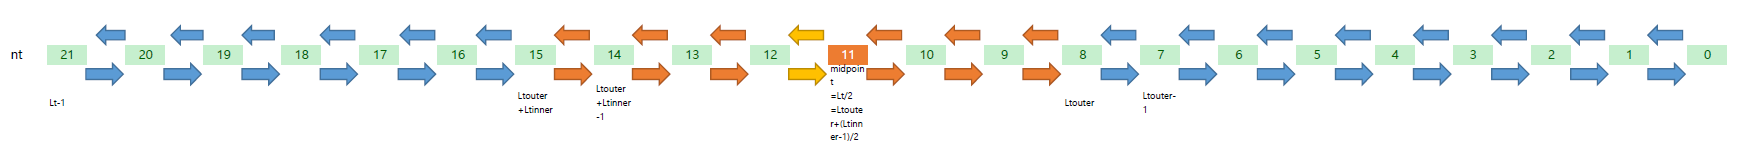
\includegraphics[width=1.0\linewidth]{fig_transfer_matrix}
	\caption{Time evolution of state vectors in case Ltouter$=$8 and Ltinner$=$7.
		In this case, midpoint is nt$=11=$Lt/2$=$2$*$Ltouter+(Ltinner-1)/2.
		Note that {\bf pinhole\_mask} acts at the midpoint. 
		The blue arrow represents a transfer matrix with only SU(4) interaction,
		while the orange arrow represents the full transfer matrix. 
		The Yellow arrow is a full transfer matrix if {\bf ndtskip}$=$0,
		or identity if {\bf ndtskip}$=$1. 	
	}
	\label{fig:figtransfermatrix}
\end{figure}

\begin{lstlisting}[frame=single]
SUBROUTINE getzvecs(s,q_hop,zvecs,zvecsinit, &
           pinhole_mask, &
           nx_1,ny_1,nz_1, &
           nt2,nt1,ndtskip,Vwall,&
           tpion,ztau2x2,ntrim,nfillall,nc_1,zpsi_1)

DIMENSION s(0:L-1,0:L-1,0:L-1,0:Lt-1)
DIMENSION s_smear(0:L-1,0:L-1,0:L-1,0:Lt-1)
DIMENSION temp(0:L-1,0:L-1,0:L-1,0:Lt-1)
DIMENSION q_hop(0:L-1)
DIMENSION zvecs(0:L-1,0:L-1,0:L-1,0:Lt,0:1,0:1,0:n_f-1)
DIMENSION zvecsinit(0:L-1,0:L-1,0:L-1,0:1,0:1,0:n_all-1)
DIMENSION ztemp1(0:L-1,0:L-1,0:L-1,0:1,0:1,0:n_f-1)
DIMENSION ztemp2(0:L-1,0:L-1,0:L-1,0:1,0:1,0:n_f-1)
DIMENSION pinhole_mask(0:L-1,0:L-1,0:L-1,0:1,0:1)
DIMENSION ntrim(0:n_all-1)
DIMENSION nfillall(0:n_f-1,0:n_ch-1)
DIMENSION nx_1(0:n_f-1)
DIMENSION ny_1(0:n_f-1)
DIMENSION nz_1(0:n_f-1)
DIMENSION Vwall(0:L-1,0:L-1,0:L-1)
DIMENSION tpion(0:L-1,0:L-1,0:L-1,Ltouter:Ltouter+Ltinner-1,1:3)
DIMENSION zpi2x2(0:1,0:1)
DIMENSION zsS2x2(0:1,0:1)
DIMENSION zsI2x2(0:1,0:1)
DIMENSION zsSI2x2(0:1,0:1,0:1,0:1)
DIMENSION ztau2x2(0:1,0:1,0:9)
\end{lstlisting} 
\begin{itemize}
	\item computes {\bf zvecs} from {\bf zvecsinit} at {\bf nt1} until {\bf nt2}.
	\item (input) {\bf s} is a auxiliary field
	\item (input) {\bf q\_hop} is a 1-D hopping operator $\Delta(n_S)$
	\item (input) {\bf zvecsinit} is an initial waves at $nt=nt1$.
	\item (input) apply transfer matrix zvecs(nt)=M(s,nt-1)zvecs(nt-1) from nt1 
	              to Lt/2, but skip {\bf ndtskip} (i.e., set M=1) when 
	              nt is in between Lt/2, Lt/2+ndtskip. 
	              After this, apply transfer matrix until {\bf nt2}.		
	\item (output) {\bf zvecs} is all vectors generated by acting transfer matrix.
	\item (input) {\bf pinhole\_mask} is a masking the position of A-nucleons
	              which have specific spin and isospin. (?)
	\item (input) {\bf nx\_1,ny\_1,nz\_1} are central position of each nucleon in initial state. 
	               this should be updated in case of multichannel or pinhole algorithm case...
	\item (input) {\bf Vwall} is a wall potential as a function of distance of two nucleon
	\item (input) {\bf tpion} is a true pion fields 
	\item (input) {\bf ztau2x2} is a combination of $[\tau_I]_{ij} $.
	\item (input) {\bf ntrim} is a time nt where nucleon is inserted. 
	\item (input) {\bf nfillall} is a storage of index for initial waves for nucleon in each channels.
	\item (input) {\bf nc\_1}  is a channel number of initial channel
	\item (input) {\bf zpsi\_1} is a normalization factor for the first particle np=0. So that,
	              zvecs(np=0)= zvecsinit(np=0 )*zpsi\_1. But why ?                           
\end{itemize}
\begin{lstlisting}[frame=single]
!   nt2 > nt1
!....
! skipping 
!  definition of  w0,w1,w2,w3 for improved action 
!.... 
!... pp is a maximum momentum 
IF (mod(L,2) == 0) THEN
  pp = pi
ELSE
  pp = (L-1)*pi/L
END IF

! copy zvecsnit into zvecs(nt1)
! but adjust central position of each particle in zvecsinit 
! as origin in zvecs(nt1)
!
! since each single particle wave functions of nucleons does not interact,
! and the system have translational invariance, there is no problem of 
! shifting central position of each nucleon.  
! 
!...loop over ni,ns,nz,ny, nx 
  DO np = 0,0
    zvecs(nx,ny,nz,nt1,ns,ni,np) = zvecsinit(mod(nx-nx_1(np)+L,L), &
                               mod(ny-ny_1(np)+L,L), &
                               mod(nz-nz_1(np)+L,L), &
                               ns,ni,nfillall(np,nc_1))*zpsi_1           
  END DO
  DO np = 1,n_f-1
    zvecs(nx,ny,nz,nt1,ns,ni,np) = zvecsinit(mod(nx-nx_1(np)+L,L), &
                               mod(ny-ny_1(np)+L,L), &
                               mod(nz-nz_1(np)+L,L), &
                               ns,ni,nfillall(np,nc_1))
  END DO
!... end loop over ni,ns,nz,ny, nx 

!... apply pinhole_mask 
IF (nt1 .eq. int(Lt/2) .and. mask_pinhole .eq. 1) THEN
! loop over np,ni,ns,nz,ny,nx 
   zvecs(nx,ny,nz,nt1,ns,ni,np) = zvecs(nx,ny,nz,nt1,ns,ni,np)
                                  *pinhole_mask(nx,ny,nz,ns,ni)      
! end loop 
END IF

\end{lstlisting}
\begin{itemize}
	\item When copying {\bf zvecsinit(nt1)} into {\bf zvecs(nt1)}, one adjust the 
	      central position of each nucleon to be the origin. 
	      And also, {\bf zpsi\_1} is multiplied for {\bf np=0}.
	\item In case of nt1 is already at middle time, Lt/2 and {\bf mask\_pinhole=1},
	      multiply filtering {\bf pinhole\_mask(nx,ny,nz,ns,ni)}.          
\end{itemize} 

\begin{lstlisting}[frame=single]
! acting transfer matrix for zvecs(nt-1)-> zvecs(nt) 
DO nt = nt1+1, nt2
  ! set SU4 interaction 
  IF (nt <= Ltouter .OR. nt >= Ltouter+Ltinner+1) THEN
    c0_cSU4 = cSU4
  ELSE
    c0_cSU4 = c0
  END IF
  ! copy auxilary s(nt-1) to temp 
  DO nz = 0,L-1; DO ny = 0,L-1; DO nx = 0,L-1
    temp(nx,ny,nz,nt-1) = s(nx,ny,nz,nt-1)
  END DO; END DO; END DO
  ! obtain smeared s_smear(nt-1) from initial s(nt-1)
  call do_smear_u(s_smear(0,0,0,nt-1), &
    temp(0,0,0,nt-1), &
    1.D0,smearNLL,smearNLL2,smearNLL3,smearNLL4)

  DO np = 0,n_f-1

    IF (nt <= ntrim(nfillall(np,nc_1)) &
       .OR. (nt-1 >= Lt/2 .AND. nt-1 < Lt/2+ndtskip)) THEN

       !...loop over nx,ny,nz,ns,ni
       zvecs(nx,ny,nz,nt,ns,ni,np) = zvecs(nx,ny,nz,nt-1,ns,ni,np)

    ELSE
        ! apply the :1-H_{free}: to zvecs 
        !...loop over nx,ny,nz,ns,ni
        zvecs(nx,ny,nz,nt,ns,ni,np)= zvecs(nx,ny,nz,nt-1,ns,ni,np)+... 
        
        ! compute  <0|a_{NL}(n) |zvecs(nt-1)> -> smeared ztemp1 
        !
        DO ni = 0,1; DO ns = 0,1
          call do_smear(ztemp1(0,0,0,ns,ni,np), &
             zvecs(0,0,0,nt-1,ns,ni,np), &
             1.D0,smear)
        END DO; END DO

        ! loop over ni,ns,nz,ny,nx
        !  
          ztemp1(nx,ny,nz,ns,ni,np) =  &
                 ztemp1(nx,ny,nz,ns,ni,np) &
                 *dsqrt(-c0_cSU4*atovera)  &
                 *s_smear(nx,ny,nz,nt-1)
        ! end loop over ni,ns,nz,ny,nx
        

        ! add  :(1-H_free): term and :-V_{s}: term 
        DO ni = 0,1; DO ns = 0,1
           call do_reverse_smear(zvecs(0,0,0,nt,ns,ni,np), &
                 ztemp1(0,0,0,ns,ni,np), 1.D0,smear)
        END DO; END DO

    END IF
  END DO
\end{lstlisting}
\begin{itemize}
	\item refer the fist note for the details of each steps.
	\item This corresponds to computing 
	 $$|zvecs_{nt}\ra= (1-H_{free})|zvecs_{nt-1}\ra -V_s|zvecs_{nt-1}\ra$$
\end{itemize}



\begin{lstlisting}[frame=single]
! ******
! The first Ltouter time steps and last Ltouter time 
! steps are done using only the SU(4) contact interaction ...
! for Ltinner time steps, add pion contributions
  IF (nt >= Ltouter+1 .AND. nt <= Ltouter+Ltinner) THEN
    !..loops
       zsSI2x2(ns,nss,ni,nii) = 0.D0                         
    !..end loops    
    DO iso = 1,3
      ! set pi1, pi2 , pi3 = 0.D0, 1,2,3 is a spin index
      ! pi1 = sum_nn Delta_1(nn) pi_I(n+nn)
      do nn = 0,L-1
         pi1 = pi1 &
              + q_hop(nn)*tpion(MOD(nx+nn,L),ny,nz,nt-1,iso)
         pi2 = pi2 &
              + q_hop(nn)*tpion(nx,MOD(ny+nn,L),nz,nt-1,iso)
         pi3 = pi3 &
              + q_hop(nn)*tpion(nx,ny,MOD(nz+nn,L),nt-1,iso)
      enddo
      ! zpi2x2 = [sigma_S] pi_{SI}
      zpi2x2(0,0) = pi3
      zpi2x2(1,1) = -pi3
      zpi2x2(0,1) = pi1 - (0.D0,1.D0)*pi2
      zpi2x2(1,0) = pi1 + (0.D0,1.D0)*pi2
      DO nii = 0,1; DO ni = 0,1
      DO nss = 0,1; DO ns = 0,1
          zsSI2x2(ns,nss,ni,nii) = zsSI2x2(ns,nss,ni,nii) &
              - gA*atovera/(2.D0*fpi)*zpi2x2(ns,nss) &
              * ztau2x2(ni,nii,iso)                          
      END DO; END DO
      END DO; END DO
    END DO
    
    DO np = 0,n_f-1
      IF (nt > ntrim(nfillall(np,nc_1)) &
         .AND. (nt-1 < Lt/2 .OR. nt-1 >= Lt/2+ndtskip)) THEN

        DO nii = 0,1; DO ni = 0,1
        DO nss = 0,1; DO ns = 0,1                                  
           zvecs(nx,ny,nz,nt,ns,ni,np) = zvecs(nx,ny,nz,nt,ns,ni,np) &
              + zsSI2x2(ns,nss,ni,nii) &
              *zvecs(nx,ny,nz,nt-1,nss,nii,np)            
        END DO; END DO
        END DO; END DO      
      END IF
    END DO
    END DO; END DO; END DO  

  END IF

 !... apply pinhole mask if nt1< Lt/2 <= nt2  
  IF (nt .eq. int(Lt/2) .and. mask_pinhole .eq. 1) THEN
    DO np = 0,n_f-1
    DO ni = 0,1; DO ns = 0,1      
    DO nz = 0,L-1; DO ny = 0,L-1; DO nx = 0,L-1                              
     zvecs(nx,ny,nz,nt,ns,ni,np) = &
         zvecs(nx,ny,nz,nt,ns,ni,np) &
         *pinhole_mask(nx,ny,nz,ns,ni)      
    END DO; END DO; END DO
    END DO; END DO
    END DO
  END IF   

END DO

END SUBROUTINE getzvecs
\end{lstlisting} 

\begin{itemize}
	\item derivative coupling of pion is done by using $\Delta_S(n_S)$ function. 
	\item $\sum_{n'} \Delta_S(n')\pi_I(\vn+n'_S)$ is named pi1,pi2,pi3 and it is used to
	     compute $\left[\sigma_1*pi1+\sigma_2*pi2+\sigma_3*pi3\right]_{s1,s2}$
	     for given isospin. 
	
\end{itemize}


\subsection{Coulomb correction} 

Suppose {\bf zvecs} and {\bf zdualvecs} are already computed and we want to 
compute the correction of perturbative Coulomb potential to binding energy.
In principle, we may insert the Coulomb  



\chapter{MATLAB code} 

Here, let us try to understand the MATLAB code for 2-body calculation. 

In the MATLAB code, matrix KK represent the matrix elements $\la \vn| \hat{K}|\vn'\ra $
for all lattice points $|\vn\ra$
\bea 
\hat{K}=\frac{\alpha_t}{2m}\sum_{k=0,1,2\dots}(-1)^k w_k \sum_{\vn}\sum_{\hat{l}=1,2,3}
             \left[a^\dagger(\vn)a(\vn+k\hat{l})+  a^\dagger(\vn)a(\vn-k\hat{l})\right] 
\eea 
By using  
\bea 
\la \vn_i| \sum_{\hat{l}}\sum_{\vn}  a^\dagger(\vn) a(\vn\pm k\hat{l})|\vn_j\ra 
=\sum_{\hat{l}}\delta_{\vn_j, \vn_i\pm k\hat{l}}
\eea 
One can construct the matrix $\la \vn|\hat{K}|\vn\ra$ by summing matrix such like 
$k_{ij}= \delta_{\vn_j,\vn_i+\hat{1}},\dots$. 

\end{document}
